%%%%%%%%%%%%%%%%%%%%%%%%%%%%%%%%%%%%%%%%%%%%%%%%%%%%%%%%%%%%%%%%%%%%%%%%%%%%%%%
% Chapter 2 - Simultaneous Imaging of Cerebral Blood Flow and Oxygen Tension
%%%%%%%%%%%%%%%%%%%%%%%%%%%%%%%%%%%%%%%%%%%%%%%%%%%%%%%%%%%%%%%%%%%%%%%%%%%%%%%

\chapter{Simultaneous Imaging of Cerebral Blood Flow and Oxygen Tension}

Measurements of hemodynamic parameters in cerebral vasculature have been invaluable in preclinical research for understanding the physiology of the normal and diseased brain. The combination of imaging techniques to simultaneously measure multiple hemodynamic parameters has become increasingly common and used to study stroke \cite{Jones:2008gb}, cortical spreading depression \cite{Sakadzic:2009jo}, and functional brain activation \cite{Dunn:2005gw, Dunn:2003wy}. Advancements in computer processing power and the increased availability of lasers and light-emitting diodes across a diverse range of wavelengths have facilitated the development of these multi-parameter hemodynamic imaging platforms.

In 2010, Ponticorvo and Dunn \cite{Ponticorvo:2010uv} detailed a dual-modality imaging system capable of simultaneously measuring cerebral blood flow (CBF) and oxygen tension (\ce{pO2}) in cortical vasculature. The system combined laser speckle contrast imaging (LSCI) and oxygen-dependent quenching of phosphorescence. An unpublished modification to the system added multispectral reflectance imaging for measurements of oxy- and deoxyhemoglobin \cite{Ponticorvo:2010ur}. The primary innovation of this design was the use of a digital micromirror device (DMD) to achieve spatial localization of the phosphorescent signal. A DMD is an optical semiconductor device that consists of a two-dimensional array of thousands of individually addressable mirrors that can be tilted to spatially modulate light. By patterning excitation light, phosphorescence could be constrained to only the targeted regions of interest, which allowed the use of high sensitivity point detectors. This overcame the traditional limitations of spatially-resolved phosphorescence imaging that either required the use of expensive laser scanning systems \cite{Yaseen:2009ep, Kazmi:2013ey} or exposure-gated cameras \cite{Shonat:2003ia, Sakadzic:2009jo}.

However, a major limitation of this system was the phosphorescent probe Oxyphor R2 \cite{Dunphy:2002tz}, which required conjugation with albumin in order to remain stable \textit{in vivo}. The system was also optically limited to only targeting large regions of the field of view for \ce{pO2} measurements and was incapable of performing multiple actions simultaneously with the DMD. This chapter details a redesign of the system by Ponticorvo and Dunn \cite{Ponticorvo:2010uv} with the goal of improving the spatial and temporal resolutions of both imaging modalities through implementation of newer hardware and a more robust oxygen-sensitive phosphorescent probe.



%%%%%%%%%%%%%%%%%%%%%%%%%%%%%%%%%%%%%%%%%%%%%%%%%%%%%%%%%%%%%%%%%%%%%%%%%%%%%%%
% Section 2.1 - Instrumentation
%%%%%%%%%%%%%%%%%%%%%%%%%%%%%%%%%%%%%%%%%%%%%%%%%%%%%%%%%%%%%%%%%%%%%%%%%%%%%%%
\section{Instrumentation}

The following dual-modality imaging system combines LSCI with oxygen-dependent quenching of phosphorescence for the simultaneous measurement of CBF and \ce{pO2}. Because LSCI is rarely light-limited, the optical design is focused on the projection of patterned excitation light off the DMD and the efficient collection of the emitted phosphorescence. The spectral cutoffs for the system were dictated by the new phosphorescent probe, Oxyphor PtG4 \cite{Esipova:2011hi}, an oxygen-sensitive dendritic probe that contains Platinum(II)-\textit{meso}-tetra-(3,5-dicarboxyphenyl)tetrabenzoporphyrin (PtTBP) as the phosphorescent core. Unlike its predecessors Oxyphor R2 and G2 \cite{Dunphy:2002tz}, which were limited to albumin-rich environments for stability, Oxyphor PtG4 is encapsulated within a hydrophobic dendrimer and PEGylated to increase solubility and biocompatibility. These modifications provide increased stability across a wider range of temperatures and pH values and eliminate the need for conjugation with blood proteins \cite{Esipova:2011hi}. Oxyphor PtG4 has two excitation maxima near 435 nm (Soret) and 623 nm (Q band) and a broad emission spectra peaking at 782 nm (Figure \ref{fig:oxyphor_ptg4}A). The probe was calibrated under physiological conditions (37 $^\circ$C, pH 7.2) by measuring the phosphorescent decay lifetime ($\tau$) as the environmental \ce{pO2} was increased from 0 mmHg to 160 mmHg (Figure \ref{fig:oxyphor_ptg4}B). The unquenched lifetime ($\tau_0$) is 47 $\mu$s in an oxygen-free environment.

% Figure - Oxyphor PtG4 Spectra + Calibration
\begin{figure}
    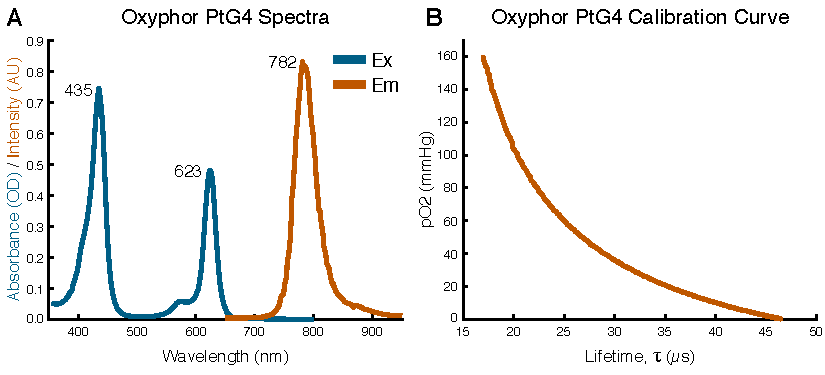
\includegraphics{figures/chapter_2/oxyphorptg4.pdf}
    \caption {
        \label{fig:oxyphor_ptg4}
        \textbf{(A)} Excitation (blue) and emission (red) spectra for Oxyphor PtG4. \textbf{(B)} Calibration curve relating environmental \ce{pO2} to the measured phosphorescence lifetime ($\tau$) under physiological conditions (37 $^\circ$C, pH 7.2).
    }
\end{figure}

%%%%%%%%%%%%%%%%%%%%%%%%%%%%%%%%%%%%%%%%%%%%%%%%%%%%%%%%%%%%%%%%%%%%%%%%%%%%%%%
\subsection{Optical System}

The schematic of the optical system can be seen in Figure \ref{fig:systemschematic_1}. The excitation and emission spectra of Oxyphor PtG4 dictated laser selection and dichroic beamsplitter cutoff wavelengths. LSCI was performed using a 685 nm laser diode (50 mW, HL6750MG, Thorlabs, Inc.) illuminating the sample at an oblique angle. The laser was mounted in a temperature-controlled housing (TCLDM9, Thorlabs, Inc.) and collimated with a slight divergence using an aspheric lens (C240TME-B, Thorlabs, Inc.) to illuminate the entire field of view. The operating current was set using a laser diode controller (LDC202, Thorlabs, Inc.) and the diode temperature regulated using a temperature controller (TED200C, Thorlabs, Inc.). The scattered light was relayed through a pair of dichroic beamsplitters and a bandpass filter (685$\pm$40 nm, S685/40m, Chroma Technology Corp.) to a CMOS camera (acA1300-60gmNIR, 1280 x 1024 pixels, Basler AG) with 2x magnification for a field of view of 3.5 x 2.8 mm. The camera was controlled via the Basler Pylon API using custom software written in C++ (i.e. the "Speckle Software").

% Figure - System Schematic (Ver. 1)
\begin{figure}
    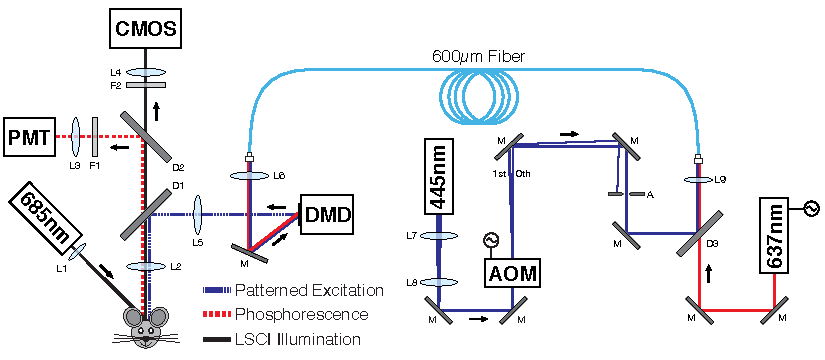
\includegraphics{figures/chapter_2/systemschematic.pdf}
    \caption {
        \label{fig:systemschematic_1}
        Schematic of the dual-modality imaging system.
    }
\end{figure}

Separately, two different lasers at 445 nm and 637 nm were selected to target the Soret and Q band excitation maxima of Oxyphor PtG4. Each laser can be used independently to collect phosphorescence lifetime measurements with different penetration depths and sample volumes because of their wavelengths. The 445 nm laser (200 mW, AixiZ) is a packaged device with a 4 mm collimated output that operates at a fixed current with convection cooling. The beam size was reduced to 1 mm and gated using an 80 MHz acousto-optic modulator (23080-2-LTD AOM and 21080-1AM RF Driver, Neos Technologies, Inc.). The 637 nm laser diode (250 mW, HL6388MG, Thorlabs, Inc.) was mounted in a temperature-controlled housing (LDM21, Thorlabs, Inc.) and collimated using an aspheric lens (C330TME-B, Thorlabs, Inc.). The laser was directly gated using its driver (LDD400-1P, Wavelength Electronics, Inc.) and the diode temperature regulated using an external temperature controller (300B, Newport Corp.). Both lasers were gated via analog modulation to produce 20 $\mu$s pulses of light for time domain lifetime measurements.

The lasers were coaligned using a dichroic beamsplitter (DMLP490, Thorlabs, Inc.) and coupled into a fiber optic patch cord (P600-2-VIS-NIR, Ocean Optics, Inc.) with a 600 $\mu$m core size. The modulated laser light was relayed to the primary imaging system via the patch cord and re-collimated to illuminate the DMD. A DLP LightCrafter Evaluation Module (Texas Instruments) was modified to expose the bare DMD (DLP3000, 608 x 684 pixels, 7.6 $\mu$m pitch) for illumination. The spatially patterned modulated light was then relayed to the sample with 0.5x magnification to selectively excite Oxyphor PtG4 for lifetime measurements.

The emitted phosphorescence was separated from the excitation and scattered LSCI laser light using a pair of dichroic beamsplitters (650 nm, ZT640rdc, Chroma Technology and 750 nm, FF750-SDi02, Semrock, Inc.) and a bandpass filter (810$\pm$90 nm, ET810/90m, Chroma Technology Corp.) and relayed to a photomultiplier tube for detection (H7422P-50, Hamamatsu Photonics K.K.). Figure \ref{fig:systemspectra} contains an overview of the spectral separation in the imaging system and Table \ref{tab:filters} details each filter in the primary imaging path.

% Figure - System Spectra
\begin{figure}
    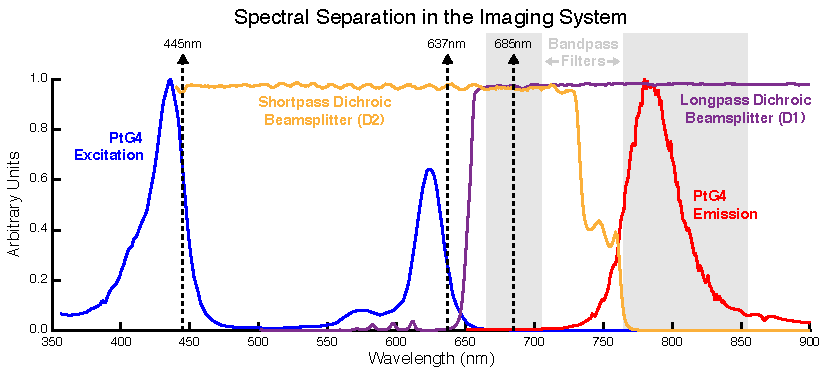
\includegraphics{figures/chapter_2/systemspectra.pdf}
    \caption {
        \label{fig:systemspectra}
        Dichroic beamsplitters and bandpass filters used to spectrally separate light in the imaging system. A longpass dichroic beamsplitter (purple) separates the excitation lasers (445 and 637 nm) from the scattered LSCI laser (685 nm) and Oxyphor PtG4 phosphorescence emission (red). A shortpass dichroic beamsplitter (gold) separates the LSCI light from the phosphorescence for detection. Bandpass filters (shaded grey) limit ambient and scattered light from reaching the detectors. All values are normalized.
    }
\end{figure}

% Table - Filter Summary
\begin{table}
    \caption{Summary of optical filters.}
    \label{tab:filters}
    \centering
    \resizebox{\textwidth}{!}{
    \begin{tabular}{ccccc} \addlinespace \toprule
        \thead{Label} & \thead{Filter} & \thead{Usage} & \thead{Manufacturer} & \thead{Part Number} \\ \midrule
        \textbf{D1} & \makecell{650 nm longpass \\ dichroic beamsplitter} & \makecell{Excitation \\ Separation} & Chroma & ZT640rdc \\ \hline
        \textbf{D2} & \makecell{750 nm shortpass \\ dichroic beamsplitter} & \makecell{Emission \\ Separation} & Semrock & FF750-SDi02-25x36 \\ \hline
        \textbf{D3} & \makecell{490 nm longpass \\ dichroic beamsplitter} & \makecell{Laser \\ Coalignment} & Thorlabs & DMLP490 \\ \hline
        \textbf{F1} & \makecell{810$\pm$90 nm \\ bandpass} & \makecell{Phosphorescence \\ Isolation} & Chroma & ET810/90m \\ \hline
        \textbf{F2} & \makecell{685$\pm$40 nm \\ bandpass} & \makecell{LSCI \\ Isolation} & Chroma & S685/40m \\ \bottomrule
    \end{tabular}}
\end{table}



%%%%%%%%%%%%%%%%%%%%%%%%%%%%%%%%%%%%%%%%%%%%%%%%%%%%%%%%%%%%%%%%%%%%%%%%%%%%%%%
\subsection{Laser Speckle Contrast Imaging}

\blindtext

%%%%%%%%%%%%%%%%%%%%%%%%%%%%%%%%%%%%%%%%%%%%%%%%%%%%%%%%%%%%%%%%%%%%%%%%%%%%%%%
\subsection{Phosphorescence Lifetime Measurements}

\blindtext



%%%%%%%%%%%%%%%%%%%%%%%%%%%%%%%%%%%%%%%%%%%%%%%%%%%%%%%%%%%%%%%%%%%%%%%%%%%%%%%
% Section 2.2 - Static Oxygen Tension Measurements in Cuvettes
%%%%%%%%%%%%%%%%%%%%%%%%%%%%%%%%%%%%%%%%%%%%%%%%%%%%%%%%%%%%%%%%%%%%%%%%%%%%%%%
\section{Static Oxygen Tension Measurements in Cuvettes}

\blindtext



%%%%%%%%%%%%%%%%%%%%%%%%%%%%%%%%%%%%%%%%%%%%%%%%%%%%%%%%%%%%%%%%%%%%%%%%%%%%%%%
% Section 2.3 - Demonstration of Acute In Vivo Imaging
%%%%%%%%%%%%%%%%%%%%%%%%%%%%%%%%%%%%%%%%%%%%%%%%%%%%%%%%%%%%%%%%%%%%%%%%%%%%%%%
\section{Demonstration of Acute In Vivo Imaging}

\blindtext



%%%%%%%%%%%%%%%%%%%%%%%%%%%%%%%%%%%%%%%%%%%%%%%%%%%%%%%%%%%%%%%%%%%%%%%%%%%%%%%
% Section 2.4 - Discussion
%%%%%%%%%%%%%%%%%%%%%%%%%%%%%%%%%%%%%%%%%%%%%%%%%%%%%%%%%%%%%%%%%%%%%%%%%%%%%%%
\section{Discussion}

\blindtext



%%%%%%%%%%%%%%%%%%%%%%%%%%%%%%%%%%%%%%%%%%%%%%%%%%%%%%%%%%%%%%%%%%%%%%%%%%%%%%%
% END Chapter 2
%%%%%%%%%%%%%%%%%%%%%%%%%%%%%%%%%%%%%%%%%%%%%%%%%%%%%%%%%%%%%%%%%%%%%%%%%%%%%%%
